The Bode plot of the plant $P(s)$, and the loop gain with PD control $P(s)C_{PD}(s)$, and the loop gain with PID control $P(s)C_{PID}(s)$ are shown in Figure~\ref{fig:hw_mass_bode_specs}.
\begin{figure}[H]
   \centering
   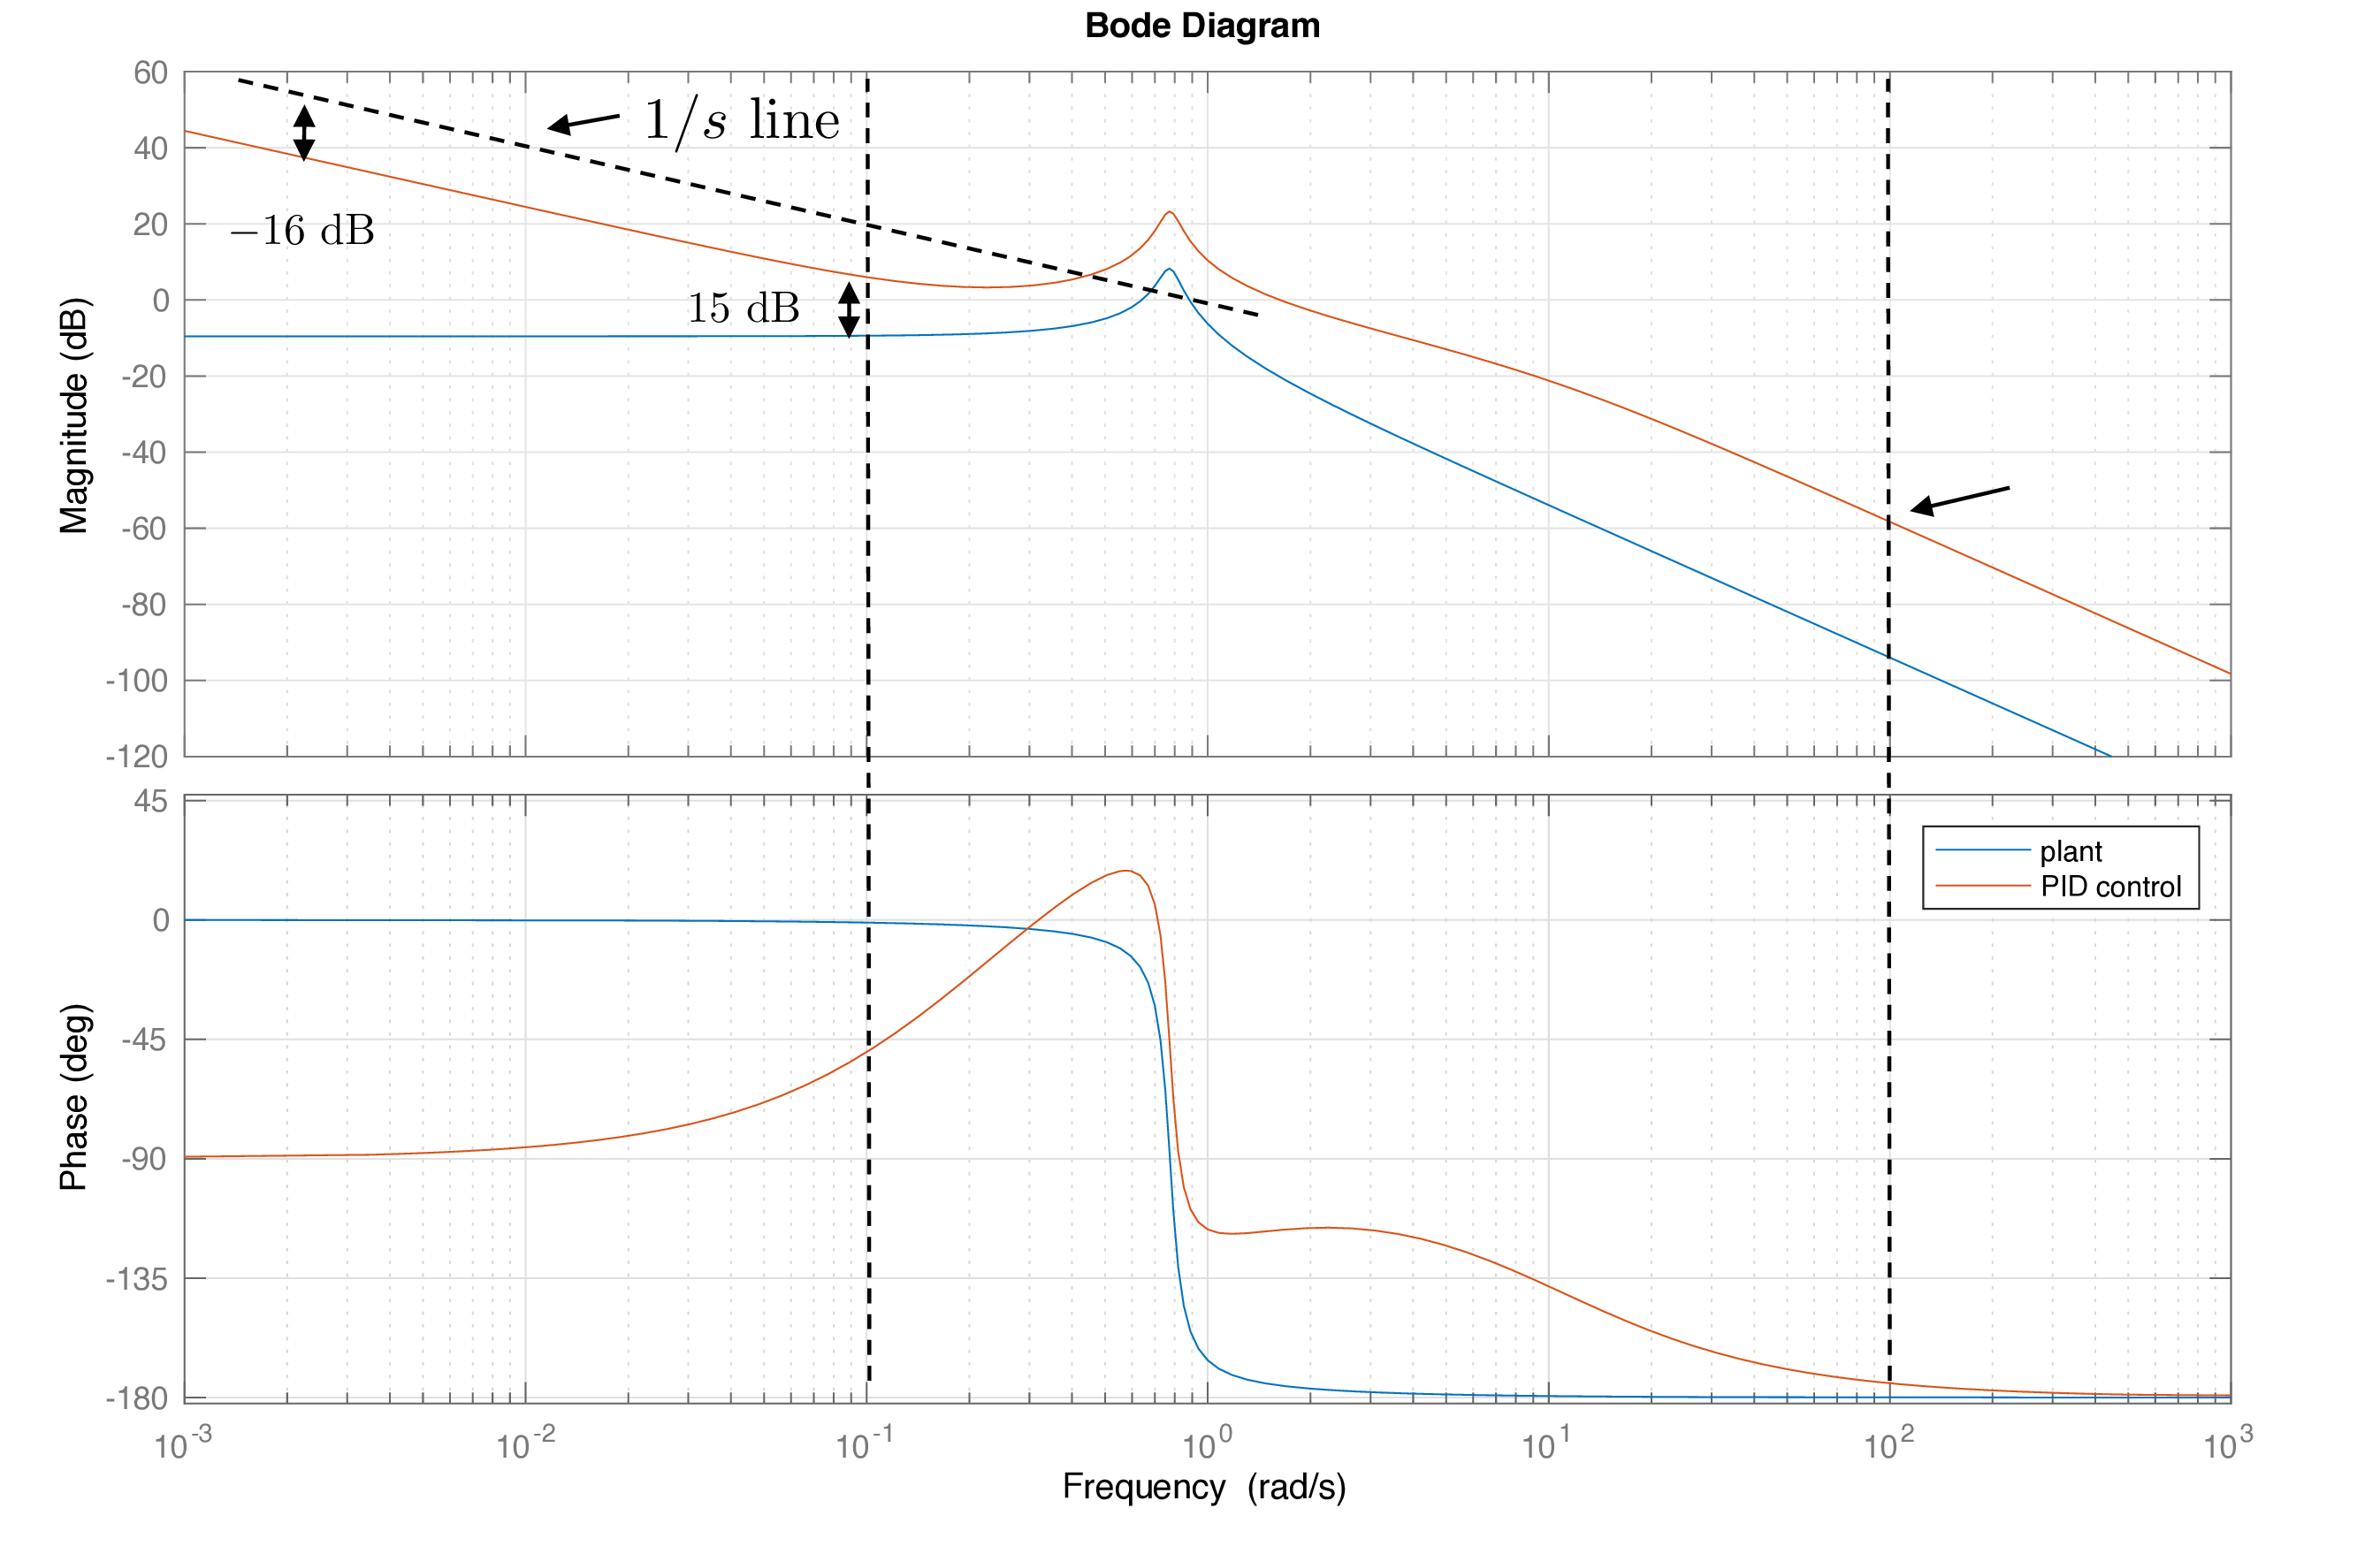
\includegraphics[width=0.95\textwidth]{6_design_studies/figures/hw_mass_bode_specs.pdf}
   \caption{Bode plot for mass spring damper, plant only, and under PID control.}
   \label{fig:hw_mass_bode_specs}
\end{figure}



{\bf (a)} From Figure~\ref{fig:hw_mass_bode_specs} we see that as $\omega\to 0$, the Bode magnitude for PID control satisfies $20\log_{10}\abs{P(j\omega)C(j\omega)}-20\log_{10}\abs{\frac{1}{j\omega}}\to B_1=-16$~dB.  
Therefore, the steady state tracking error is
\[
\lim_{t\to\infty} \abs{e(t)} = \frac{1}{M_v},
\]
where $M_v=10^{B_1/20}=0.1585$, which implies that the steady state error is $6.3096$.

{\bf (b)} For  $\omega\leq\omega_{d_{in}} = 0.1$~rad/s, we have 
\[
20\log_{10}\abs{P(j\omega)C_{PD}(j\omega)}-20\log_{10}\abs{P(j\omega)}\to B_{d_{in}}=15\text{~dB}.
\]
Therefore, 
\[
\gamma_{d_{in}} = 10^{-15/20} = 0.1778,
\]
implying that 18\% of the input disturbance will show up in the output.

{\bf (c)} For $\omega\geq\omega_n=100$~rad/sec, we see from Figure~\ref{fig:hw_mass_bode_specs} that $B_{no} = -58$~dB.  Therefore, $\gamma_n = 10^{-58/20} = 0.0013$ which implies that $0.13$\% of the noise will show up in the output signal.